\PassOptionsToPackage{unicode}{hyperref}
\documentclass[t]{beamer}

\usepackage[
  orientation=portrait,
  size=a0,
  scale=1.0,
]{beamerposter}

\usetheme{tudoposter}

\usepackage{fontspec}

%\usepackage{polyglossia}
%\setmainlanguage{german}
\usepackage[english]{babel}

\usepackage{csquotes}
\usepackage{microtype}
\usepackage{mathtools}

\usepackage{blindtext}

\usepackage{multicol}
\setlength{\columnsep}{1em}

\usepackage{xfrac}

\usepackage{tikz}
\usetikzlibrary{shapes, arrows, backgrounds, fit, tikzmark, arrows.meta, calc, quotes, angles}

\usepackage[center]{caption}

\usepackage{siunitx}

\usepackage[export]{adjustbox}

\usepackage{xcolor}
\usepackage{listings}
\lstset{
  commentstyle=\color{black!60},    % comment style
}

\lstdefinestyle{base}{
  moredelim=**[is][\color{black!30}]{@}{@},
}

\usepackage{mdframed} %nice frames
\definecolor{light-gray}{gray}{0.95} %the shade of grey that stack exchange uses

\usepackage{graphicx}

% Evaluate at command
\NewDocumentCommand{\evalat}{sO{\big}mm}{%
  \IfBooleanTF{#1}
   {\mleft. #3 \mright|_{#4}}
   {#3#2|_{#4}}%
}


%% this is used to create an inline bibliography
\usepackage[backend=biber, style=numeric, sorting=none]{biblatex}
\addbibresource{biblatex-phys.bib}

\DeclareFieldFormat*{title}{\textit{#1}}
\renewcommand*{\bibfont}{\footnotesize}
\defbibenvironment{bibliography}
  {\noindent}
  {\unspace}
  {}

\renewbibmacro*{begentry}{%
  \usebeamercolor{bibliography item}%
  \color{bibliography item.fg}%
  \printtext[labelnumberwidth]{%
    \printfield{prefixnumber}%
    \printfield{labelnumber}%
  }%
  \setunit{\addnbspace}%
}
\renewcommand*{\finentrypunct}{\addperiod\space}

\newlength{\thirdtextwidth}
\setlength\thirdtextwidth{0.333333\textwidth}

\newlength{\itemseparation}
\setlength\itemseparation{0.25em}

\title{High-energy lepton and photon simulations with the framework PROPOSAL}
\author{Jean-Marco Alameddine$^{1}$, Pascal Gutjahr$^{1}$}
\institute[ETH]{$^{1}$TU Dortmund University, Otto-Hahn-Str. 4a, 44227 Dortmund, Germany}
\date{4. Juli 2015}

\titlegraphic{%
  
\includegraphics[width=1.0\linewidth, left]{tudo.pdf}\\
  %\vspace{0.2em}
  %
\includegraphics[width=0.8\linewidth, left]{BUW.png}\\
  %\vspace{0.2em}
  %
\includegraphics[width=1.0\linewidth, left]{dfg_logo_englisch_blau_en.jpg}
}

\begin{document}


  \begin{columns}[onlytextwidth]%
    \begin{column}{0.45\textwidth}%
      \begin{block}[equal height group=F]{Introduction to PROPOSAL}%
  \begin{itemize}
    \setlength\itemsep{\itemseparation}
    \item Monte Carlo simulations are crucial to train machine learning algorithms
    \begin{itemize}
      \setlength\itemsep{\itemseparation}
      \item[$\rightarrow$] The underlying tools need to be both precise and performant
    \end{itemize}
    \item PROPOSAL is a simulation framework, providing 3D Monte Carlo simulations of high-energy electrons, positrons, muons, taus and photons \cite{koehne2013proposal, dunsch_2018_proposal_improvements}
    \item Different parametrizations of physical processes, including up-to-date parametrizations, are available
    \item High-performance and high-precision simulations, optimized for large-scale particle propagation
    \item PROPOSAL is actively maintained. Recent updates include:
    \begin{itemize}
      \item[$\rightarrow$] Improvements in the simulation of photons by including photoproduction, photoeffect, and muon pair production (relevant for low-energy and very-high-energy photons)
      \item[$\rightarrow$] Code restructuring and modularization, so PROPOSAL can be used as a framework by providing individual modules
    \end{itemize}
  \end{itemize}

      \vspace{0.8em}
              \begin{center}
                \colorbox{light-gray}{
            \begin{minipage}[ht]{0.75\linewidth}
              \begin{center}
              \textbf{Find the PROPOSAL repository under:}\\ \url{github.com/tudo-astroparticlephysics/PROPOSAL} %\vspace{0.5em}\\
              \end{center}
            \end{minipage}
            \begin{minipage}[ht]{0.24\linewidth}
              \centering
                
\includegraphics[width=0.66\linewidth, valign=t]{plots/qr_proposal_transparent.png}
            \end{minipage}
                }
              \end{center}

      \end{block}%
    \end{column}%

    \begin{column}{0.55\textwidth}%
      \begin{block}[equal height group=F]{How to use PROPOSAL}%
        \begin{itemize}
          \setlength\itemsep{\itemseparation}
          \item PROPOSAL can be used as a C\texttt{++} or a Python library
            \begin{itemize}
              \setlength\itemsep{\itemseparation}
              \item[$\rightarrow$] Simple Python installation with \colorbox{tuYellow}{\texttt{pip install proposal}}
              \item[$\rightarrow$] C\texttt{++} installation using the package manager Conan and CMake
            \end{itemize}
          \item Information about the configuration environment can be read using a JSON file
        \end{itemize}
        \vspace{-0.75em}
        \begin{columns}[onlytextwidth]
        \begin{column}{0.48\textwidth}
        \begin{mdframed}[backgroundcolor=light-gray, roundcorner=10pt,leftmargin=1, rightmargin=1, innerleftmargin=15, innertopmargin=15,innerbottommargin=15, outerlinewidth=1, linecolor=light-gray]

          \lstinputlisting[
          language=Python,
          basicstyle=\footnotesize\ttfamily,
          style=base,
          escapechar=\$,
          breaklines=true
          ]{code/example.txt}
          \end{mdframed} 

          \end{column}
          \begin{column}{0.07\textwidth}
          \begin{center}
            \vspace{7.5em}
            \begin{tikzpicture}
            \draw[
              -triangle 90,
               line width=4mm,
                postaction={draw, line width=0.7cm, shorten >=1cm, -}
            ] (0,0) -- (2,0);
          \end{tikzpicture}
          \end{center}          
        \end{column}
          \begin{column}{0.45\textwidth}
            \begin{figure}
              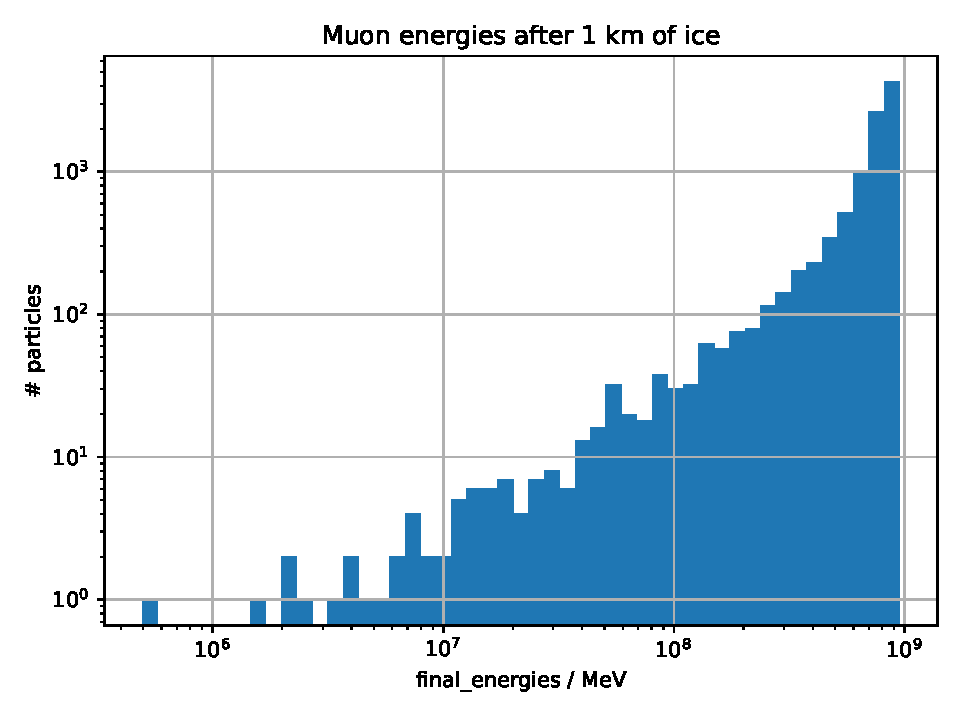
\includegraphics[width=\linewidth, height=.4\textheight, keepaspectratio]{plots/example_output.pdf}
            \end{figure}
          \end{column}
        \end{columns}

      \end{block}%
    \end{column}%    
  \end{columns}%

  \begin{columns}[onlytextwidth]%
    \begin{column}{\textwidth}%
    \begin{block}[equal height group=J]{Simulation of Deflection Uncertainties on Direction Reconstructions of Muons Using PROPOSAL}%
      \begin{columns}[onlytextwidth]
        \begin{column}{0.33\textwidth}

        There are two types of scattering interactions for muon propagation:
      \vspace{0.5em}

        \textbf{1. Multiple scattering:} (figure adapted from \cite{dunsch})

        \begin{figure}
          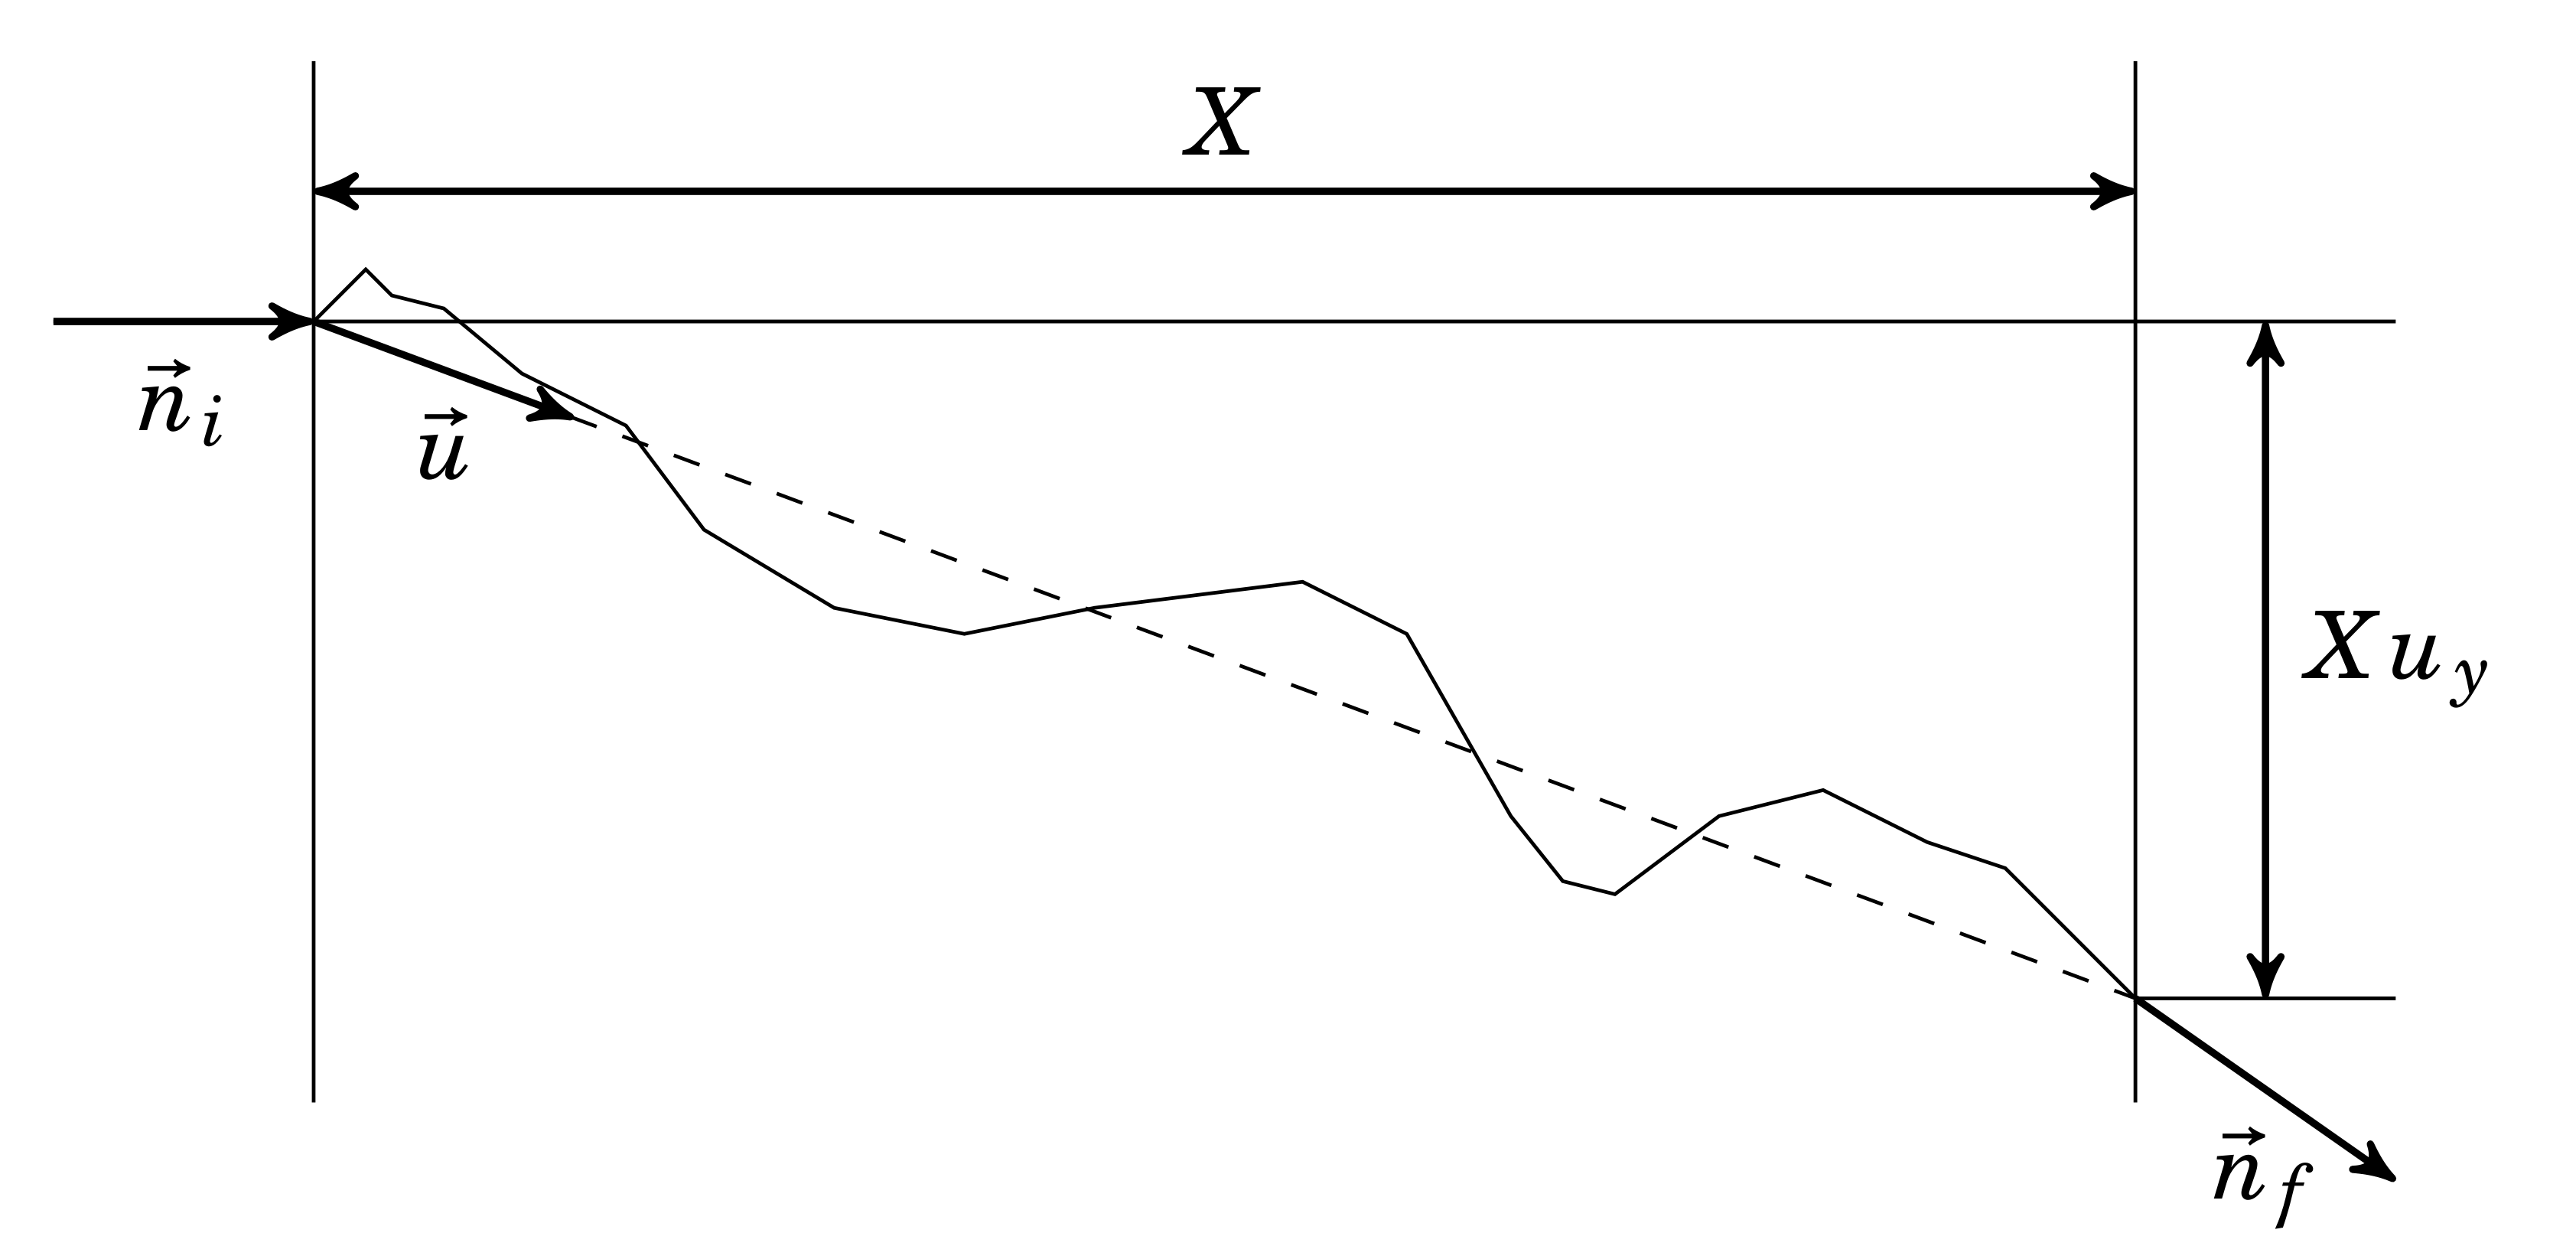
\includegraphics[width=0.7\linewidth, height=.4\textheight, keepaspectratio]{plots/multiple_scattering_dunsch.png}
        \end{figure}

        \begin{itemize}
          \item[$\rightarrow$] Described by Molière theory or a Gaussian approximation
          \item[$\rightarrow$] Relevant contribution, especially at low energies
        \end{itemize}

      \vspace{0.5em}

        \textbf{2. Stochastic deflections:}

        \begin{figure}
            \begin{tikzpicture}[scale=2.5, every node/.style={scale=1.0}]
                \centering

                \coordinate (start) at (-1,0);
                \coordinate (kink) at (1.8, 0);
                \coordinate (end) at (4.5, 0.8);
                \coordinate (continue) at (4.5, 0);



                \draw [black, line width=0.6mm] (start) -- node[above] {$\mu$}  (kink);
                \draw [->, black, line width=0.6mm] (kink) -- node[above] {$\mu^\prime$}  (end);
                \draw [black, dashed, line width=0.2mm] (kink) -- (continue);

                \fill [red] (kink) circle (0.15) node[label=below: $\substack{\text{stochastic} \\ \text{interaction}}$]{};

                \pic [draw, "$\theta$", angle eccentricity=0.7, angle radius=3.3cm] {angle = continue--kink--end};

            \end{tikzpicture}
            %\caption*{Visualization of stochastic muon deflections.}
        \end{figure} 

        \begin{itemize}
          \item[$\rightarrow$] Deflection of initial particle in individual interaction
          \item[$\rightarrow$] Might be a contribution for highly stochastic energy losses
        \end{itemize}


          \end{column}
          \begin{column}{0.33\textwidth}  


            \textbf{Summary of arXiv:2208.11902 \cite{gutjahr2022}:}
            \vspace{0.5em}

            \textbf{Motivation:}
            \begin{itemize}
              \setlength\itemsep{\itemseparation}
              \item Directional reconstruction of muons is essential for applications such as neutrino astronomy or muon tomography
              \begin{itemize}
                \item[$\rightarrow$] In this paper, we have analyzed muon deflections based on simulations with PROPOSAL
              \end{itemize}
            \end{itemize}
            \textbf{Methods:} 
            \begin{itemize}
              \setlength\itemsep{\itemseparation}
              \item As a cross check, comparisons of PROPOSAL simulations with \textsc{Geant4}, MUSIC, and experimental measurements were performed
              \begin{itemize}
                \item[$\rightarrow$] They show a good agreement
              \end{itemize}
              \item We performed simulations of muons with idential initial energies, and plotted the accumulated muon deflections for different final energies (see Figure on the right)
            \end{itemize}
            \textbf{Results:}
            \begin{itemize}
                \setlength\itemsep{\itemseparation}
                \item The accumulated deflection primarily depends in the final muon energy and is independent of the initial energy
                \item Compared to the angular resolutions of current and future neutrino telescopes, we can see a potential impact of muon deflections on the angular resolution of KM3NeT at energies $E_\text{f} \leq \SI{1}{\tera\electronvolt}$
            \end{itemize}
            %\vspace{0.5em}

             % \begin{center}
             %   \colorbox{tuYellow}{
             %     \begin{minipage}[ht]{0.85\linewidth}
             %       \begin{itemize}
             %       \item[$\rightarrow$] The accumulated deflection primarily depends on the final muon energy and is independent of the initial energy
             %       \item[$\rightarrow$] Compared to the angular resolutions of current and future neutrino telescopes, we can see a potential impact of muon %deflections on the angular resolution of KM3NeT at energies $E_\text{f} \leq \SI{1}{\tera\electronvolt}$%
             %     \end{itemize}%
             %     \end{minipage}%
             %   }
             % \end{center}


           \end{column}
          \begin{column}{0.33\textwidth}
            \begin{figure}
              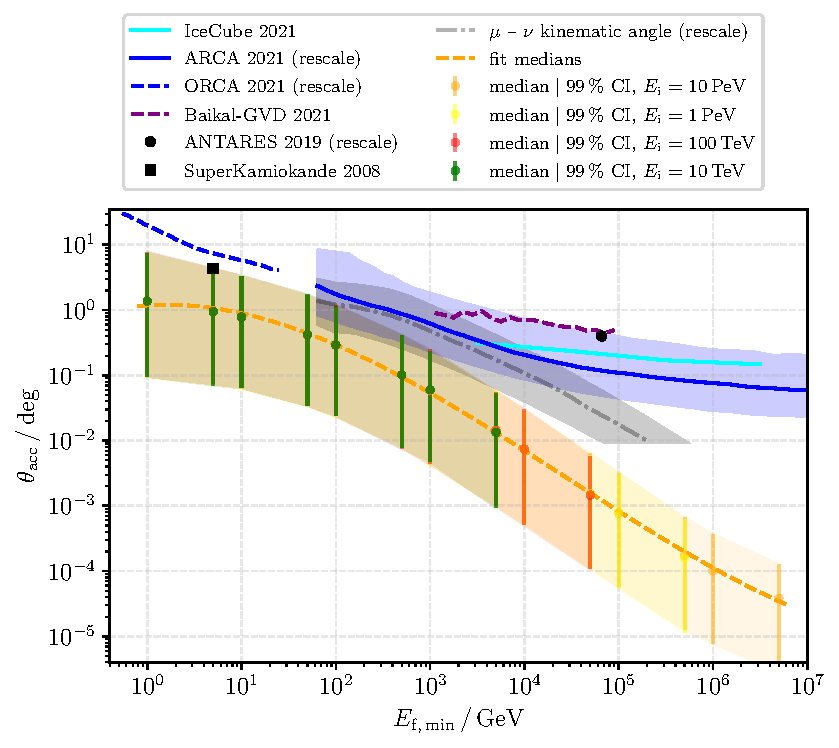
\includegraphics[width=0.9\linewidth, height=.4\textheight, keepaspectratio]{plots/fit_median_defl_cut_10percent_only_poly_new_resolution_rescale_no_icecube_paper_final_all.pdf}
              \caption*{Median of the accumulated deflection $\theta_\text{acc}$ with a $\SI{99}{\percent}$ central interval for four different initial muon energies $E_\text{i}$. Simulations in ice.}
            \end{figure}
          \end{column}
      \end{columns}



    \end{block}
    \end{column}%
  \end{columns}%

  \begin{columns}[onlytextwidth]%
    \begin{column}{\thirdtextwidth}%
      \begin{block}[equal height group=B]{Application: CORSIKA~8}%
              \begin{itemize}
                \setlength\itemsep{\itemseparation}
                \item New version of the air shower simulation framework CORSIKA
                \begin{itemize}
                  \setlength\itemsep{\itemseparation}
                  \item[$\rightarrow$] Entirely new code structure, based on modern C\texttt{++} 
                  \item[$\rightarrow$] Focus on flexibility, modularity, efficiency and reliability \cite{Engel2018}
                \end{itemize}
                \item PROPOSAL is used to simulate the electromagnetic and muonic shower component
                \begin{itemize}
                  \setlength\itemsep{\itemseparation}
                  \item[$\rightarrow$] PROPOSAL provides individual modules, where each module solves specific physical tasks \cite{Alameddine_2020}
                  \item[$\rightarrow$] CORSIKA~8 uses these modules to calculate interaction lengths, energy losses, multiple scattering and secondary particles 
                \end{itemize}
                \item First comparisons of CORSIKA~8 and CORSIKA~7: Good agreement for simulations of electromagnetic showers \cite{Alameddine:2021iq}
              \end{itemize}

        \vspace{0.5em}

              \begin{figure}
                \centering
                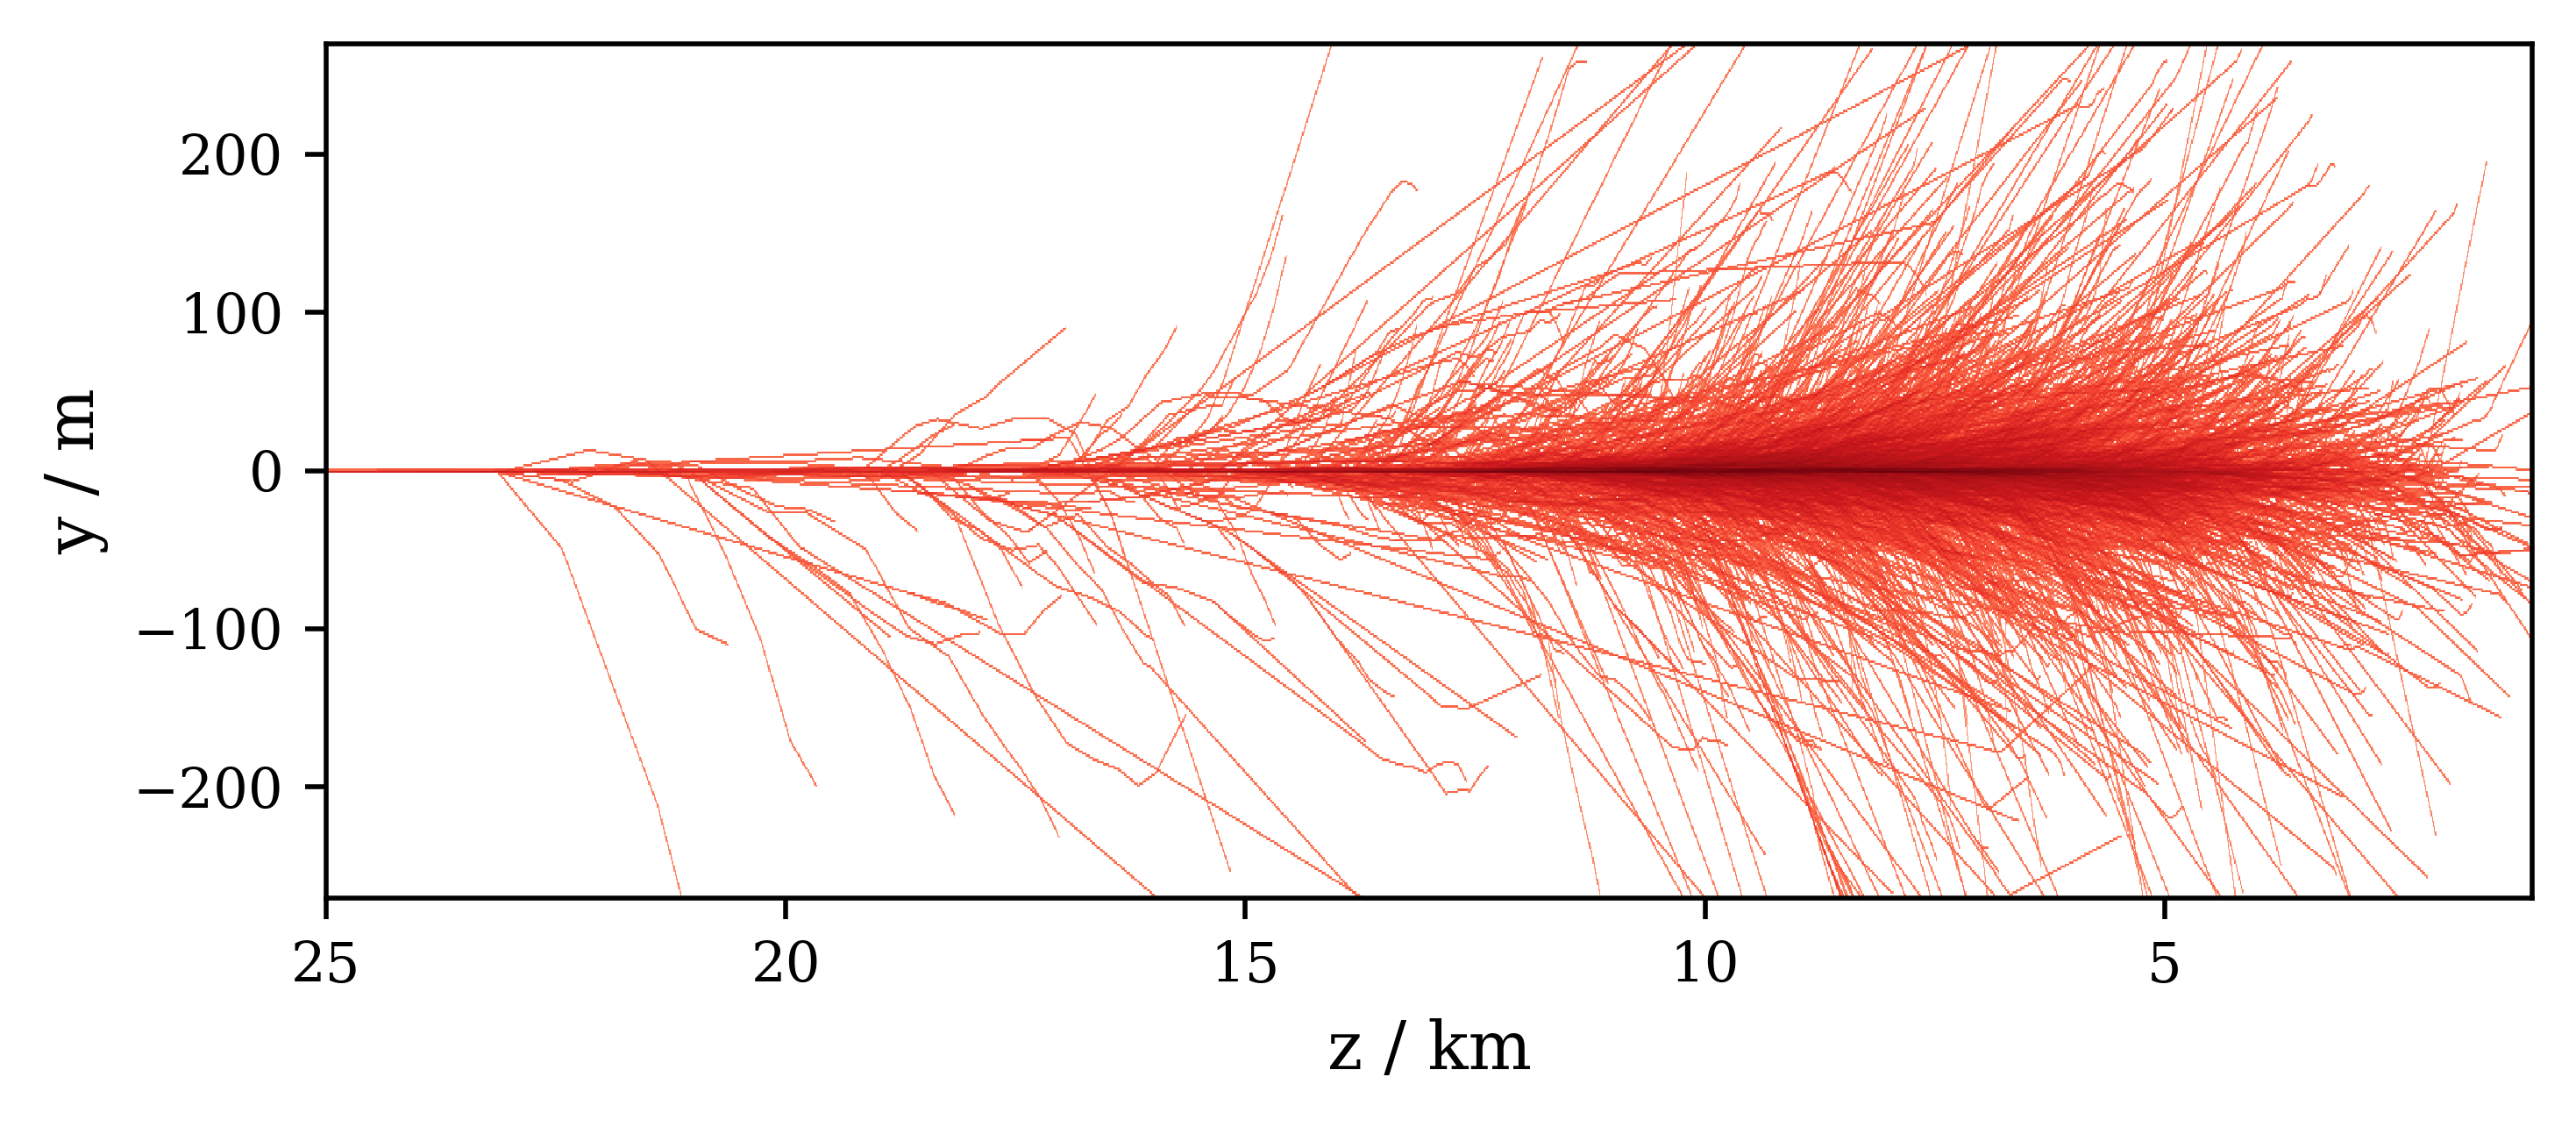
\includegraphics[width=0.8\linewidth, height=.4\textheight, keepaspectratio]{plots/shower_horizonal.png}
                \caption*{\SI{1}{\tera\electronvolt} $e^-$ shower simulated with CORSIKA~8}
              \end{figure}

              %\begin{itemize}
              %  \item[$\rightarrow$] More on CORSIKA~8 in talk by A.~Sandrock (Thursday, 5:30 PM)
              %\end{itemize}

      \end{block}%
    \end{column}%
    \begin{column}{\thirdtextwidth}%
      \begin{block}[equal height group=B]{Application: Neutrino telescopes}%
        \begin{itemize}
          \setlength\itemsep{\itemseparation}
          \item PROPOSAL is used by neutrino telescopes, for example in the IceCube Neutrino observatory or in the software framework NuRadioMC
          \item Simulation of muon and tau energy losses in ice
          \begin{itemize}
            \setlength\itemsep{\itemseparation}
            \item[$\rightarrow$] Precise simulations and an accurate description of cross sections are crucial
          \end{itemize}
        \end{itemize}

        \vspace{1.75em}

        \begin{figure}
          \centering
          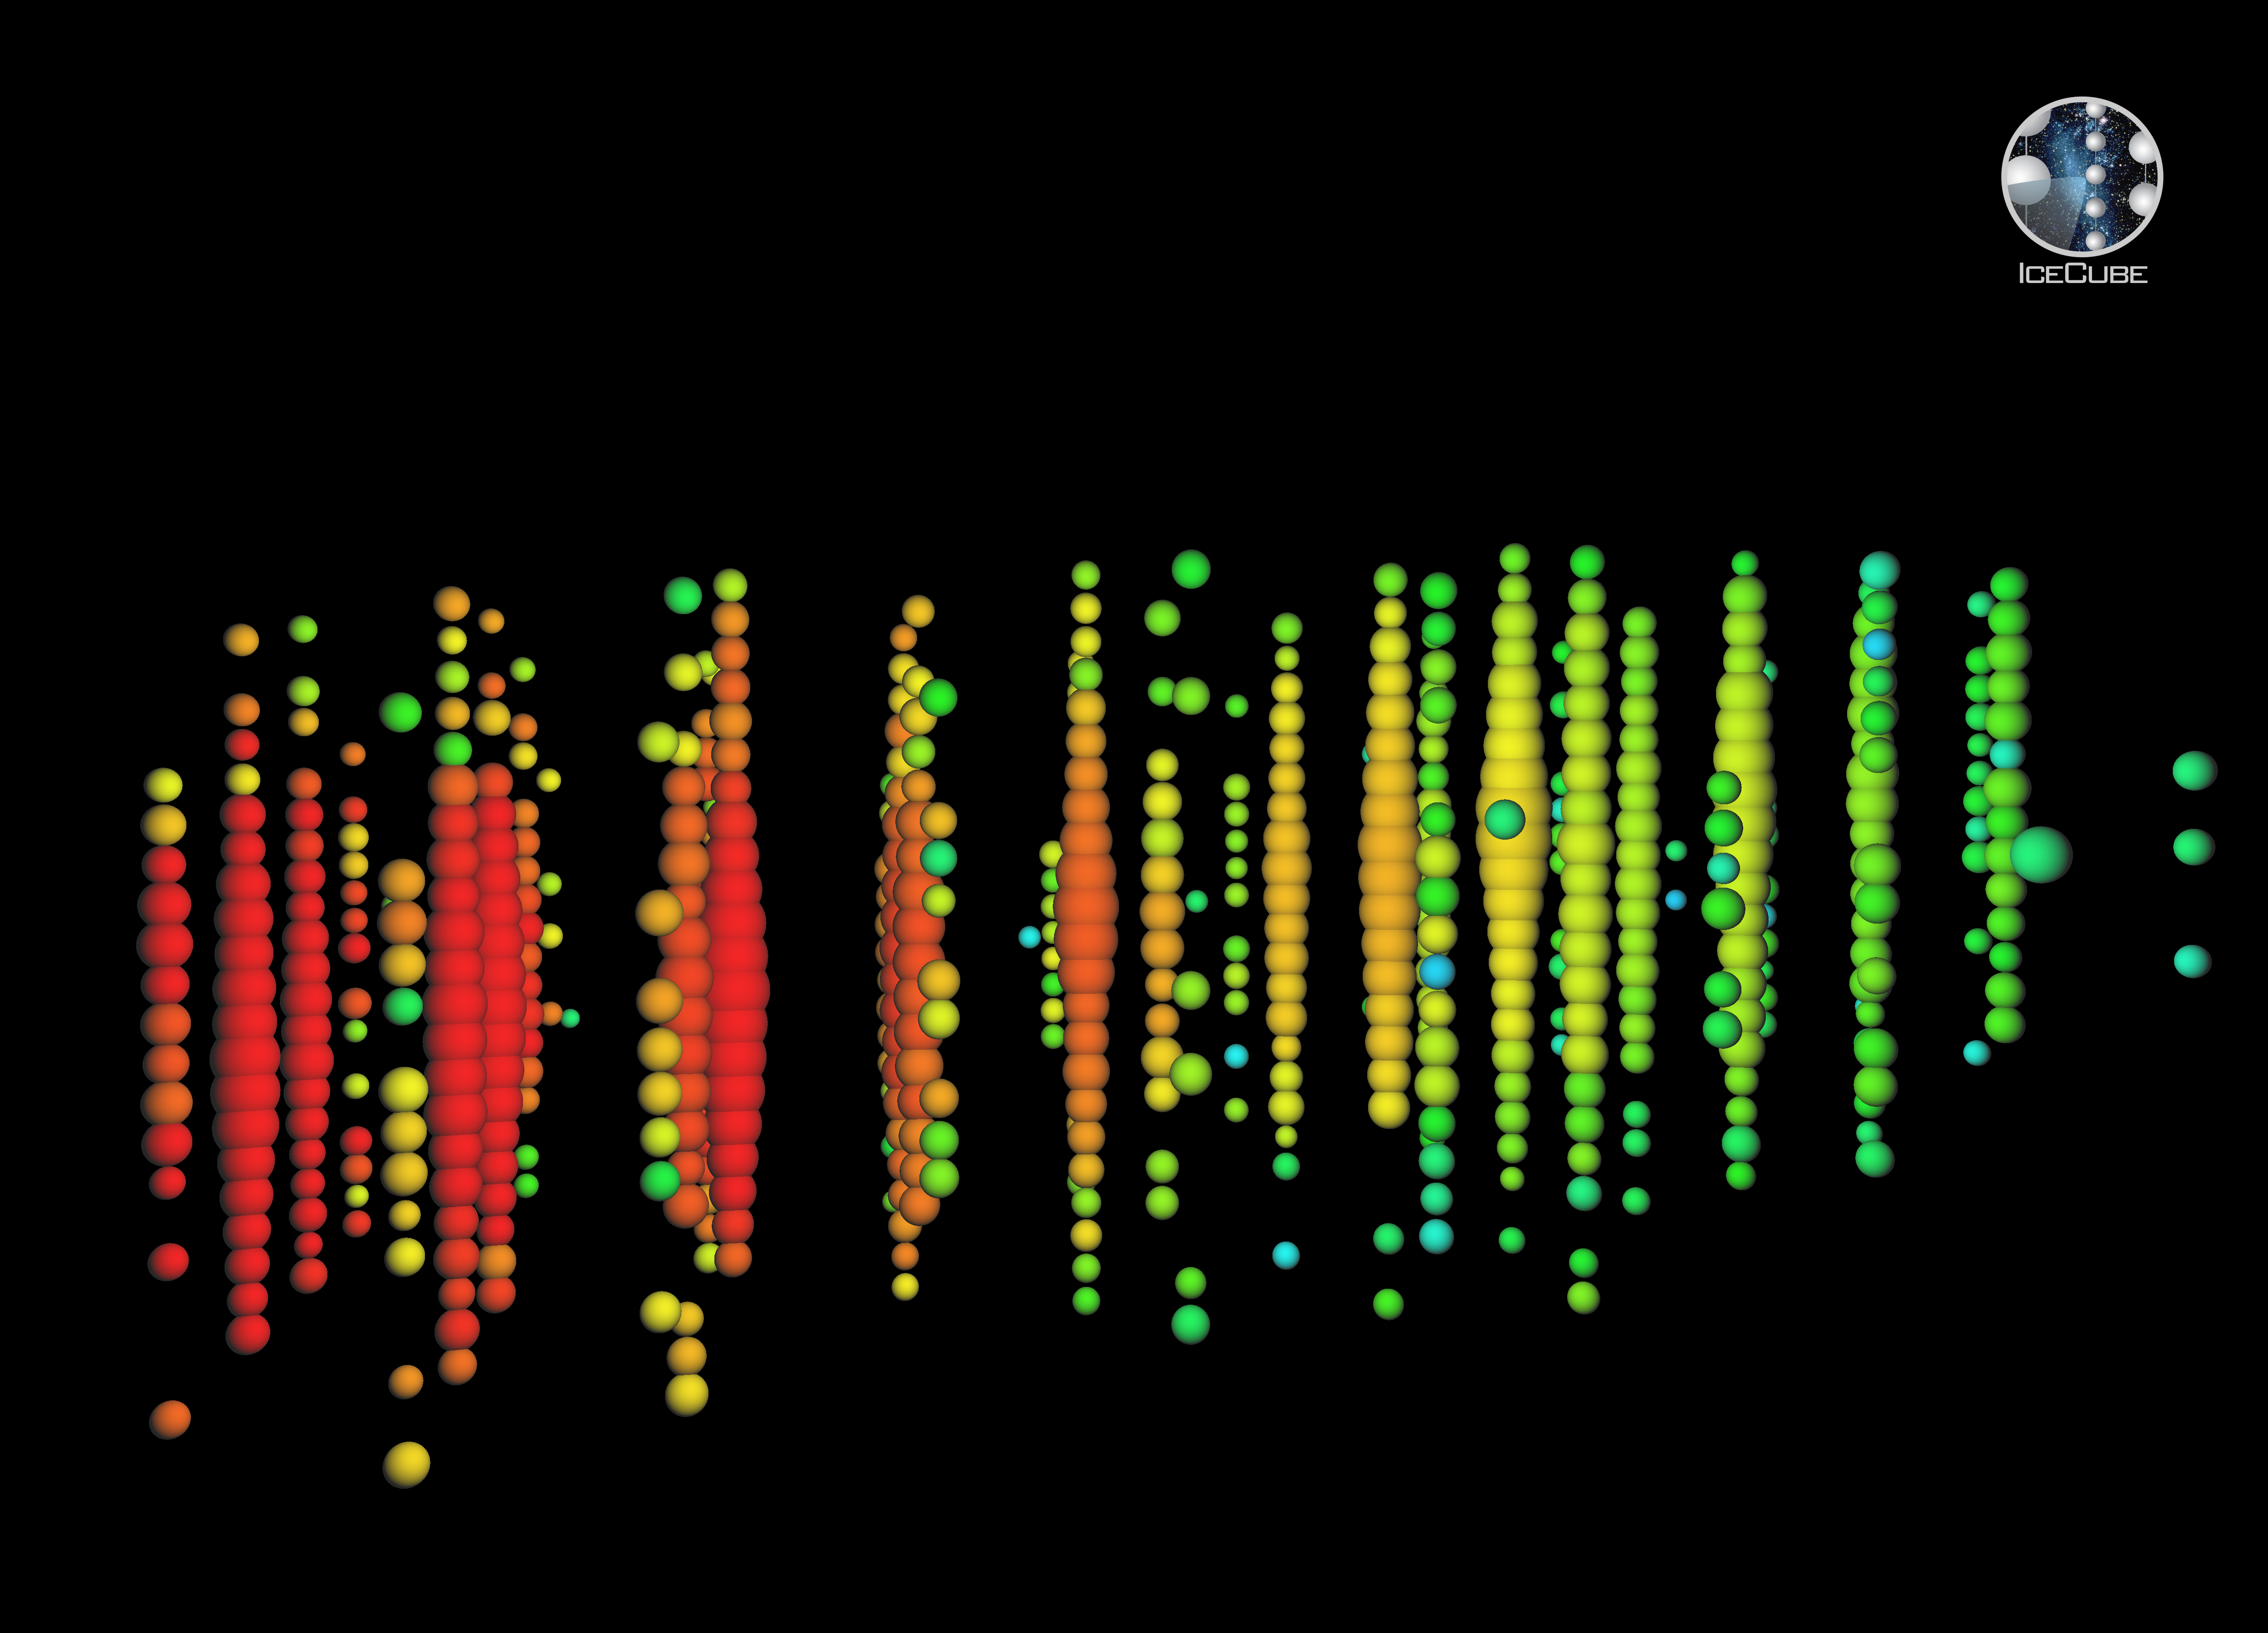
\includegraphics[width=0.7\linewidth, height=.4\textheight, keepaspectratio]{plots/icecube_muon.jpg}
          \caption*{Muon track in the IceCube detector \\(\emph{Source: IceCube Collaboration})}
        \end{figure}

      \end{block}
    \end{column}

    \begin{column}{\thirdtextwidth}%
      \begin{block}[equal height group=B]{Application: Muography}%
        \begin{itemize}
          \setlength\itemsep{\itemseparation}
          \item Non-invasive imaging technique using Cosmic Ray muons
          \item Tracing muon number along trajectories: Provides information, for example on density anomalies
          \item PROPOSAL is a well-suited tool to provide the necessary muon simulations
          \begin{itemize}
            \setlength\itemsep{\itemseparation}
            \item[$\rightarrow$] Currently analyzing the possibilities to use muography in mining with PROPOSAL simulations
          \end{itemize} 
        \end{itemize}
      \vspace{1.25em}
        \begin{figure}
            \begin{tikzpicture}[scale=2.5, every node/.style={scale=0.85}]
                \centering

                \coordinate (A) at (0, 0);

                % ground
                \draw[draw=none, fill=gray, fill opacity=1.0] ($ (A) + (-3.5,-2.5) $) rectangle ++(7, 4);

                % sky
                \draw[draw=none, fill={rgb:red,0.33;green,0.5;blue,0.98}, fill opacity=0.5] ($ (A) + (-3.5,1.5) $) rectangle ++(7, 1);
                \node[draw=none] at ($ (A) + (0.0, 2) $) {Sky};

                % mining shaft
                \draw[draw=none, fill={rgb:black,1;white,2}, fill opacity=1.0] ($ (A) + (2, -2.0) $) rectangle ++(0.25, 3.5);
                \draw[draw=none, fill={rgb:black,1;white,2}, fill opacity=1.0] ($ (A) + (-2.0, -2.0) $) rectangle ++(4, 0.5);

                \node[draw=none] at ($ (A) + (0.8, -1.75) $) {Mining shaft};

                % detector
                \node [cylinder, shape border rotate=90, draw,minimum height=0.40cm,minimum width=0.25cm, aspect=0.4] (detector) at ($ (A) + (-0.5, -1.8) $) {};

                % impurity
                \draw[draw=none,fill=black, fill opacity=0.7] ($ (A) + (0.2, -0.4) $) ellipse (0.3cm and 0.1cm);
                \node[draw=none, text width=1cm] at ($ (A) + (0.8, -0.4) $) {Anomaly};

                % muons
                \draw [densely dotted, blue, line width=0.25mm] ($ (A) + (-2.5, 2.0) $) -- ($ (detector) + (0.2, -0.5) $) node [near start, above, xshift=1ex] (TextNode) {$\mu$};

                \draw [densely dotted, blue, line width=0.25mm] ($ (A) + (-1.0, 2.0) $) -- ($ (detector) + (0.1, -0.5) $) node [near start, above, xshift=1ex] (TextNode) {$\mu$};

                \draw [densely dotted, blue, line width=0.25mm] ($ (A) + (1.0, 2.0) $) -- ($ (A) + (0.2, -0.4) $) node [pos=0.4, above, xshift=-1ex] (TextNode) {$\mu$};

            \end{tikzpicture}
            \caption*{Visualization of the muography technique}
        \end{figure} 

      \end{block}%
    \end{column}%
  \end{columns}%

  \begin{columns}[onlytextwidth]%
    \begin{column}{0.4\textwidth}%
      \begin{block}[equal height group=Z]{Outlook}%
        \begin{itemize}
          \setlength\itemsep{\itemseparation}
          \item Implementation of the LPM effect for inhomogeneous media
          \begin{itemize}
            \setlength\itemsep{\itemseparation}
            \item[$\rightarrow$] Important for very-high-energy air showers
          \end{itemize}
          \item Implementation of only-stochastic propagation
          \begin{itemize}
            \setlength\itemsep{\itemseparation}
            \item[$\rightarrow$] Allows for neutrino propagation with PROPOSAL
          \end{itemize}
        \end{itemize}
      \end{block}
    \end{column}
    \begin{column}{0.4\textwidth}%
      \begin{block}[equal height group=Z]{Contact}%
        \begin{center}
          \begin{figure}[ht]
            \begin{minipage}[ht]{0.5\linewidth}
              \textbf{Contact via mail:}

              \vspace{0.25em}
              \href{mailto:me@jean-marco.alameddine@tu-dortmund.de}{jean-marco.alameddine@tu-dortmund.de} 
              \\ \href{mailto:me@pascal.gutjahr@tu-dortmund.de}{pascal.gutjahr@tu-dortmund.de} 
            \end{minipage}
            \begin{minipage}[ht]{0.24\linewidth}
              \centering
                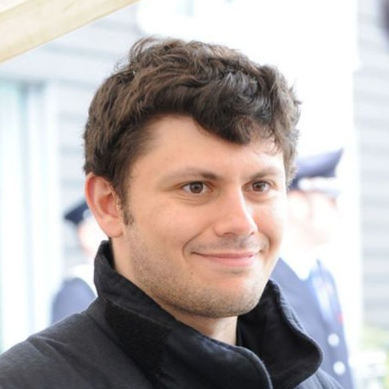
\includegraphics[width=0.61\linewidth, valign=t]{plots/ich.png}
                \caption*{\footnotesize Jean-Marco}
            \end{minipage}
              \begin{minipage}[ht]{0.24\linewidth}
              \centering
                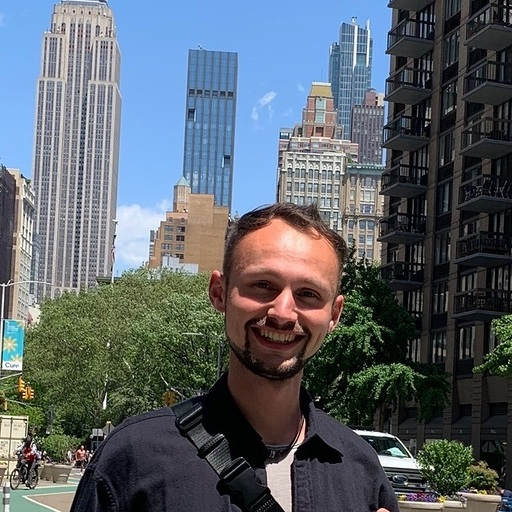
\includegraphics[width=0.61\linewidth, valign=t]{plots/pascal.jpg}
                \caption*{\footnotesize Pascal}
            \end{minipage}
          \end{figure}
        \end{center}
      \end{block}
    \end{column}
    \end{columns}

  \vspace*{\fill}
  \begin{columns}[onlytextwidth]%
    \begin{column}{0.75\textwidth}%
      \begin{alertblock}[equal height group=bottom, fonttitle=\normalsize]{References}
        \begin{multicols}{3}
          \footnotesize%
          \printbibliography%
        \end{multicols}
      \end{alertblock}
    \end{column}
    \begin{column}{0.25\textwidth}%
      \begin{alertblock}[equal height group=bottom, fonttitle=\normalsize]{Acknowledgements}
          \footnotesize%
          This work has been supported by the DFG, Collaborative Research Center SFB 876 (project C3) and Collaborative Research Center SFB 1491 as well as by the BMBF, project 05A20PEA.\\
          Furthermore, we acknowledge funding by the DFG under the grant number SA 3876/2-1.
      \end{alertblock}
    \end{column}
  \end{columns}

  %\begin{block}[equal height group=bottom, fonttitle=\normalsize]{References}
  %  \begin{multicols}{3}
  %    \footnotesize%
  %    \printbibliography%
  %  \end{multicols}
  %\end{block}
\end{document}
